%%%%%%%%%%%%%%%%%%%%%%%%%%%%%%%%%%%%%%%%%%%%%%%%%%%%%%%%%%%%%%%%%%%%%%
% writeLaTeX Example: A quick guide to LaTeX
%
% Source: Dave Richeson (divisbyzero.com), Dickinson College
% 
% A one-size-fits-all LaTeX cheat sheet. Kept to two pages, so it 
% can be printed (double-sided) on one piece of paper
% 
% Feel free to distribute this example, but please keep the referral
% to divisbyzero.com
% 
%%%%%%%%%%%%%%%%%%%%%%%%%%%%%%%%%%%%%%%%%%%%%%%%%%%%%%%%%%%%%%%%%%%%%%
% How to use writeLaTeX: 
%
% You edit the source code here on the left, and the preview on the
% right shows you the result within a few seconds.
%
% Bookmark this page and share the URL with your co-authors. They can
% edit at the same time!
%
% You can upload figures, bibliographies, custom classes and
% styles using the files menu.
%
% If you're new to LaTeX, the wikibook is a great place to start:
% http://en.wikibooks.org/wiki/LaTeX
%
%%%%%%%%%%%%%%%%%%%%%%%%%%%%%%%%%%%%%%%%%%%%%%%%%%%%%%%%%%%%%%%%%%%%%%

\documentclass[10pt,landscape]{article}
\usepackage{amssymb,amsmath,amsthm,amsfonts}
\usepackage{multicol,multirow}
\usepackage{titlesec}
\usepackage{graphics}
\usepackage{mathtools}
\usepackage{graphicx}
\usepackage{calc}
\usepackage{ifthen}
\usepackage[landscape]{geometry}
\usepackage[colorlinks=true,citecolor=blue,linkcolor=blue]{hyperref}

\DeclarePairedDelimiter\ceil{\lceil}{\rceil}
\DeclarePairedDelimiter\floor{\lfloor}{\rfloor}


\ifthenelse{\lengthtest { \paperwidth = 11in}}
    { \geometry{top=.5in,left=.5in,right=.5in,bottom=.5in} }
	{\ifthenelse{ \lengthtest{ \paperwidth = 297mm}}
		{\geometry{top=1cm,left=1cm,right=1cm,bottom=1cm} }
		{\geometry{top=1cm,left=1cm,right=1cm,bottom=1cm} }
	}
\pagestyle{empty}
\makeatletter
\renewcommand{\section}{\@startsection{section}{1}{0mm}%
                                {-1ex plus -.5ex minus -.2ex}%
                                {0.5ex plus .2ex}%x
                                {\normalfont\large\bfseries}}
\renewcommand{\subsection}{\@startsection{subsection}{2}{0mm}%
                                {-1explus -.5ex minus -.2ex}%
                                {0.5ex plus .2ex}%
                                {\normalfont\normalsize\bfseries}}
\renewcommand{\subsubsection}{\@startsection{subsubsection}{3}{0mm}%
                                {-1ex plus -.5ex minus -.2ex}%
                                {1ex plus .2ex}%
                                {\normalfont\small\bfseries}}
\makeatother
\setcounter{secnumdepth}{0}
\setlength{\parindent}{0pt}
\setlength{\parskip}{0pt plus 0.5ex}
% -----------------------------------------------------------------------

\title{Exam 1 - Cheat Sheet}

\begin{document}

\raggedright
\footnotesize

\begin{center}
     \Large{\textbf{Cheat Sheet (Exam 1)}} \\
\end{center}
\begin{multicols}{3}
\setlength{\premulticols}{1pt}
\setlength{\postmulticols}{1pt}
\setlength{\multicolsep}{1pt}
\setlength{\columnsep}{2pt}

\titlespacing{\section}{12pc}{1.5ex plus .1ex minus .2ex}{1pc}


\section{PROOFS}

\textbf{Direct-Proofs}
\textit{Directly, i.e. working forward: Assume A is true, and then show B is true.}
A direct proof is an argument to establish an implication $p \rightarrow  q$ by assuming p and constructing
a sequence of valid inferences that establish the statement q.

\textbf{Indirect-Proof}
An indirect proof also establishes an implication $p \rightarrow  q$, but does so by way of the contrapositive:
one assumes $\neg q$ and constructs an argument that $\neg p$ must follow.

\textbf{Proof by Contradiciton:}
A proof by contradiction establishes a statement p by proving $\neg p$ must be false. In particular,
one assumes $\neg p$ and shows that a contradiction arises from this assumption

\textbf{Proof by Cases}:
A proof by cases establishes a statement q by considering a number of cases $p_{1}, p_{2}, ..., p_{n}$, one
of which must hold, and showing that in each of these cases, $p_{i} \rightarrow q$.

\textbf{Existence Proof:}
An existence proof establishes a statement of the form $\exists x P(x)$. There are two kinds. A
\textbf{constructive proof} is given by providing an explicit element c and establishing $P(c)$. A \textbf{nonconstructive}
proof is any other proof of $\exists x P(x)$ that does not provide an explicit element c such that
P(c). For example, one might proceed by contradiction and show that $\forall x \neg P(x)$ is impossible.

\textbf{Uniqueness Proof}:
Mathematical theorems often assert the existence of a unique element satisfying a given predicate.
For such theorems, a uniqueness proof must be supplied. That is, one must first prove the
existence, as described above, but then one must also argue the uniqueness of the element under
discussion. In other words, after proving $\exists xP(x)$, a uniqueness proof also requires that you prove
$\forall x \forall y((P(x) ∧ P(y)) \rightarrow (x = y))$.

\textit{Note:} The converse of an implication $p \rightarrow q$ is the implication $q \rightarrow p$.


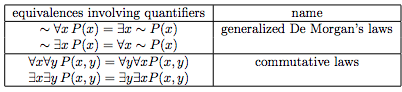
\includegraphics[scale=0.5]{de-morgans-law.png}



\subsection{Logical Equivalences}
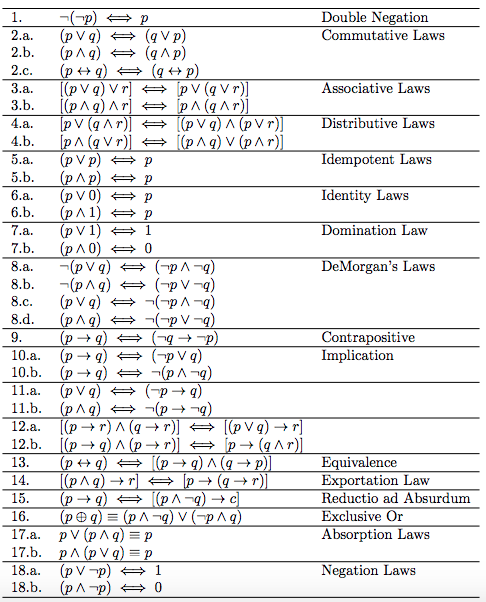
\includegraphics[scale=0.4]{logical-equivalences.png}


\subsection{Logical Implications}
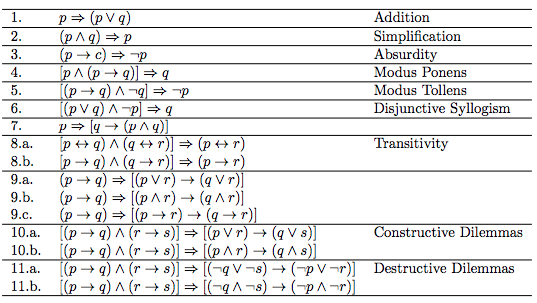
\includegraphics[scale=0.4]{logical-implications.png}

\subsection{Negations}
	\begin{enumerate}
		\item
		The contrapositive of the implication $p \rightarrow q$ is $\neg q \rightarrow \neg p$.
		
		\item
		The negation of "for every/for all" ($\forall$) is "there exits" ($\exists$).
		
		\item
		The negation of "there exists" ($\exists$) is "for every/for all" ($\forall$).
		
		\item
		The negation of "if p, then q" is "p and  $\neg$ q" (note: the negation of an "if, then" statement is NOT an "if, then" statement).
		
		\item
		The negation of "p or q" is "$\neg$p and $\neg$q".
	
		\item
		The negation of "p and q" is "$\neg$p or $\neg$q".
	\end{enumerate}

\section{SET THEORY}

\textit{Random Notes:}
The empty set is a subset of all sets.

The set $R$ \textbackslash $S = {x \in R | x \not \in S}$ is called the complement of S in R.
Sometimes $R$ \textbackslash $S$ is called the relative complement of S in R.

If A and B are nonempty finite sets, then $|A \times B| = |A| * |B|$

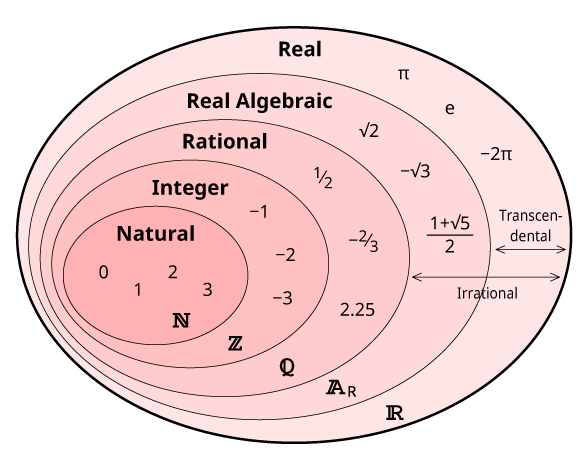
\includegraphics[scale=0.4]{number-sets.png}

$\emptyset$ – empty set \\
$\mathbb{N}$ – natural numbers \\
$\mathbb{Z}$ – integers (from Zahl, German for number).\\
$\mathbb{Q}$ – rational numbers (from quotient) \\
$\mathbb{R}$ – real numbers \\
$\mathbb{C}$ – complex numbers \\


\subsection{Set Identities} 
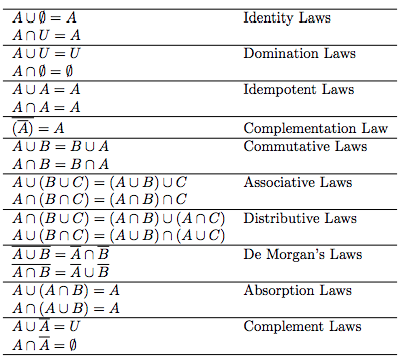
\includegraphics[scale=0.4]{set-identities.png}

\subsection{Nested / Disjoint} 

\textbf{Nested}
We call a sequence $(A_n)_{n=1}^\infty$ of sets a *nested sequence of sets* if the next set is always a subset of its predecessor, i.e.,
$$(\forall n\in\{1,2,\dots\}) A_{n+1} \subseteq A_n.$$
So the nested sequence looks like this $A_1 \supseteq A_2 \supseteq \dots \supseteq A_n \supseteq \dots$

A collection $\delta$ of sets is said to be *nested* iff for every 
$A, B \in \delta,$ 
either $A\subseteq B$ 
or $B \subseteq A.$ 
(Often you'll see 
$\delta=\lbrace A_0, A_1, A_2, \dots \rbrace$ with either 
$A_0 \subseteq A_1 \subseteq A_2 \subseteq \dots$ or $A_0 \supseteq A_1 \supseteq A_2 \supseteq\dots$, but some nested collections have a more complicated structure than those.)

So examples of nested sequences of subsets of $\mathbb R$ would be:

	\begin{enumerate}
		\item
		$A_n=(-\frac1n,\frac1n)$
		
		\item
		$A_n=[n,\infty)$
	
		\item
		$A_n=[0,1+\frac1n)$
	\end{enumerate}



\textbf{Disjoint}
A set (of sets) $\mathcal{A}$ is disjoint if $\bigcap \mathcal{A} = \emptyset$.

The set $\mathcal{A}$ is pairwise disjoint when $\forall x \in A: \forall y \in A: x \neq y \implies x \cap y = \emptyset$. This implies disjoint if $|\mathcal{A}| \ge 2$.

So $\mathcal{A} = \{x,y\}$ is disjoint iff it is pairwise disjoint.

But in maeasure theory, disjoint is often used as a shorthand for "pairwise disjoint".


\subsection{Union / Intersection}
$\bigcup_{i\in I} A_i$ is the set of all those elements which appear in \textit{some} $A_i$, and $\bigcap_{i\in I}A_i$ is the set of those elements which appear in *every* $A_i$.

\textbf{Example}
Consider the collection $C$ of intervals in $\mathbb{R}$ given by:
$C = {(5 - n, 6+1/n] | n \in \mathbb{R}}$

It is NOT \textbf{nested}, 
since 7 $\in (4, 7]$ \textbackslash 
$(3, 6 \dfrac{1}{2}]$
and 
$4 \in (3, 6 \dfrac{1}{2}]$ 
\textbackslash $(4, 7]$

(In this case, work forward from the base)

It is NOT \textbf{mutually disjoint}.

$5 \in (4,7]$ 
$\cap (3, 6 \dfrac{1}{2}] $

\textbf{Intersection:}
(4, 6]

\textbf{Union:}

$(- \infty, 7]$


\subsection{Partitions}

\textbf{Definition}: A \textit{partition} of a nonempty set $S$ is a collection $\mathfrak{C} = {B_{i}}_{i \in I}$ of nonempty mutually disjoint subsets of $S$ with $\bigcup_{i \in I} B_{i} = S. The sets B_{i} \in \mathfrak{C}$ are called \textit{blocks} of the partition.

The collection $\{\{1, 2\}, \{3, 4, 5\}, \{6\}\}$ is a partition of the set $S = \{1, 2, 3, 4, 5, 6\}$
since blocks $B_{1} = \{1,2\}, B_{2} = \{3, 4, 5\}, B_{3} = {6}$ are non-empty, mutually disjoint, and their union $\{1, 2\} \cup \{3, 4, 5\} \cup \{6\}$ is $S$.

So to show that a collection partitions a space, show that partition is:
	\begin{enumerate}
		\item
			Non-empty, or: $\forall n \in \mathbb{Z}$ \textit{(or whatever it is)}, that ${B_{i}} \neq \emptyset$. Maybe give an interval that's an element of the indexed partition.
		\item
			Disjoint,
		\item
			Spans the space given any $(x, y)$. 
	\end{enumerate}

\textbf{Example}:

For each $n \in \mathbb{Z}, let: $ \\
$\mathcal{T}_{n} = 
\{(x, y) \in 
\mathbb{R}^{2}  \mid n \leq x-y  \textless n+1\}$

Is $\mathcal{T} = \{\mathcal{T}_{n} \mid n \in \mathbb{Z}\}$ a partition of $\mathbb{R}^{2}$? Justify your answer using the definition.  \\

\textbf{Solution:} \\
	To start off, \\
	$\mathcal{T}_{0} = \{(x,y) \mid 0 \leq x-y < 1 \}$ \\
	$= \{(x,y) \mid y \leq x$ \& $y > x-1 \}$.
	
	Therefore $\mathcal{T}_{n} = \{(x,y) \mid y \leq x-n$ \& $y > x-n-1 \}$.

	\begin{enumerate}
	\item
	\textbf{Non-Empty}:  \\
	$\forall n \in \mathbb{Z}$, $\mathcal{T}_{n} \neq \emptyset$ since (0, -n) $\in \mathcal{T}_{n}$.
	
	\item
	\textbf{Disjoint}: \\
	$\forall m,n \in \mathbb{Z}$, if $m < n$, then: \\
	$\mathcal{T}_{m} \cap \mathcal{T}_{n}$ = 
	$\{(x, y) \mid m \leq x-y < m+1$ \& $n \leq x-y < n+1 \}$
	
	\item
	\textbf{Covers $\mathbb{R}^{2}$}: \\
	Given any (x,y) $\in \mathbb{R}^{2}$, let 
	$m = 
	\ceil*{x-y} \in \mathbb{Z}.$ \\
	Then $m \leq x-y < m+1$. \\
	So (x,y) $\in \mathcal{T}_{m}$. Therefore, $\mathcal{T}_{n}$'s partition
	 $\mathbb{R}^{2}$.
	
	
	\end{enumerate}
	


	
\end{multicols}

\end{document}
